\documentclass[conference]{IEEEtran}
% Include all packages from file.
% Report template for Mälardalen University
% Original template can be found: 
% https://www.overleaf.com/latex/templates/ieee-bare-demo-template-for-conferences/ypypvwjmvtdf
% Template file structure organised by: Emil Persson
% The following packages should follow the IEEE conference guidelines.

% Swedish language package 
\usepackage[utf8]{inputenc}
\usepackage[T1]{fontenc}
\usepackage[swedish,english]{babel}

% comment out stuff
\usepackage{comment}

% Long equations
\usepackage{breqn}
\usepackage{amsmath}

% Graphics
\usepackage{graphicx, float, subfigure, blindtext}

\newcommand\IEEEhyperrefsetup{
bookmarks=true,bookmarksnumbered=true,%
colorlinks=true,linkcolor={black},citecolor={black},urlcolor={black}%
}
% Preferred hyperref setup, Michael Shell
\usepackage[\IEEEhyperrefsetup, pdftex]{hyperref}

% Maths
\usepackage{mathtools}

% These packages must be at the end
\usepackage[nolist,nohyperlinks]{acronym}
\usepackage{cleveref}
\graphicspath{{images/}}
% Include acronyms
% \acrodef{acronym}[short name]{full name}
\acrodef{IC}[IC]{Integrated Circuit}
% \acrodef{svm}[SVM]{Support Vector Machine}
\newacro{svm}[SVM]{Support Vector Machine}
% Example use \ac{IC} for printing "Integrated Circuit (IC), use \ac{IC} again and it will print (IC)"
% For plural use \acp{IC} for short and \aclp{IC} for long.
% For more see: http://ftp.acc.umu.se/mirror/CTAN/macros/latex/contrib/acronym/acronym.pdf
% Include authors 
\author{\IEEEauthorblockN{
Carl Larsson\IEEEauthorrefmark{1},
Pontus Svensson\IEEEauthorrefmark{2}
}

\IEEEauthorblockA{
School of Innovation, Design and Engineering, M.Sc.Eng Robotics\\
Mälardalens University, Västerås, Sweden\\
Email:
cln20001@student.mdu.se\IEEEauthorrefmark{1}, psn19003@student.mdu.se\IEEEauthorrefmark{2}}
} 
% The report title.
\title{ELA306 Project\\
Mälardalen University - M.Sc.Eng Robotics Reports}
% Document begins here
\begin{document}
% Create the title.
\maketitle
% Example sections, name them
% according to specific needs.
\begin{abstract}
%-------------------------------------------------------------------------------------------------------------
This study covers different configurations for electric vehicles and the development of a regenerative active suspension system for the MDH solar car. A quarter car model of the system was created and simulated in Simulink and Stateflow, together with a theoretical system design. The regenerative active suspension system maintained ride comfort, however the model provided unrealistic amounts of energy regenerated and consumed. The system did show sufficient promise to warrant further research efforts.
%-------------------------------------------------------------------------------------------------------------
\end{abstract}
\begin{IEEEkeywords}
%-------------------------------------------------------------------------------------------------------------
Matlab, RASS, Regenerative active suspension system, Simulink, Stateflow
%-------------------------------------------------------------------------------------------------------------
\end{IEEEkeywords}
\section{Introduction}
\label{section:intro}

This report will first cover some electric vehicle configurations and then the modeling and simulation of a regenerative active suspension system (RASS). This project builds on previous research and heavily follows the work which has already been done by these studies\:\cite{azmiNovelOptimalControl2023} \cite{liuTransmissionEnergyharvestingStudy2021}\cite{liuModelingSimulationEnergyRegenerative2019}\cite{zhengNovelEnergyregenerativeActive2008}\cite{yinPerformanceEvaluationActive2015}\cite{okadaEnergyRegenerativeActive2007}\cite{liuModellingExperimentalStudy2016}. 

The combination of active suspension and regenerative suspension allows for maintaining the ride comfort and improving suspension performance while at the same time alleviating the major drawback of active suspension which is the energy consumption\:\cite{azmiNovelOptimalControl2023}\cite{liuTransmissionEnergyharvestingStudy2021}\cite{yinPerformanceEvaluationActive2015}. This is especially relevant for in wheel power train configurations (which the MDH solar car uses) to compensate for negative impact on the suspension system because of the increased unsprung mass\:\cite{yinPerformanceEvaluationActive2015}.

%---------------------------------------------------------------------------------------------------
% Introduktion (ca 1 sida)
%     Ge en översikt över den nuvarande situationen för elektriska fordon (EV) inom industrin, inklusive de vanligaste konfigurationerna.
%     Presentera Mälardalens Högskola (MDH) solbil, inklusive dess konfiguration och hur den skiljer sig från andra EVs.
%     Diskutera designaspekter relaterade till funktionalitet och egenskaper hos drivlinan i MDH:s solbil och andra liknande EVs.

%======================
% Introduction
%======================

%+++++++++++++++++++++++++++++++++++++++++++++++++++++++++++++++++++++++++++++++++++++++++++++++++++
% Overview

% Types
Electronic vehicles (EV) can be divided into categories depending on their power source, including: battery-powered electric vehicles (BEV), solely hybrid electric vehicles (HEV), plug-in hybrid electric vehicles (PHEV), photovoltaic electric vehicles (PEV) and Fuel-Cell Electric Vehicles (FCEV)\:\cite{hannanStateoftheArtEnergyManagement2018}\cite{khajepourElectricHybridVehicles2014}\cite{un-noorComprehensiveStudyKey2017}.
This paper is related to the MDH solar car which is a BEV and will thus focus on BEV.
Previously EV could be constructed by simply converting a non EV\:\cite{chauEVPowertrainConfigurations2014}. Modern EV are however designed from scratch to better utilize the design opportunities and flexibility offered by EV\:\cite{chauEVPowertrainConfigurations2014}\cite{othaganontMultiobjectiveOptimisationBattery2017}.

% Battery
lithium-ion (Li-ion) batteries are the most commonly used batteries in BEV\:\cite{hannanStateoftheArtEnergyManagement2018}\cite{un-noorComprehensiveStudyKey2017}\cite{chauEVPowertrainConfigurations2014}\cite{kumarDevelopmentSchemeKey2017}\cite{tahaComparativeAnalysisSingle2022}\cite{zubiLithiumionBatteryState2018}. Because of their good performance and characteristics, they are considered the best choice for EV\:\cite{hannanStateoftheArtEnergyManagement2018}. Li-ion batteries main advantages for use in BEV are their high energy density, long life, high reliability, relatively fast recharge rate and that they are lightweight\:\cite{hannanStateoftheArtEnergyManagement2018}\cite{kumarDevelopmentSchemeKey2017}\cite{zubiLithiumionBatteryState2018}. One type of lithium-ion batteries that are in high demand for BEV applications are Lithium Nickel Manganese Cobalt Oxide (LiNiMnCoO2), or NMC, batteries\:\cite{hannanStateoftheArtEnergyManagement2018}\cite{zubiLithiumionBatteryState2018}. It is common for BEV to run with multiple battery cells (90 or more) that form a battery pack rather than using one large capacity battery\:\cite{hannanStateoftheArtEnergyManagement2018}. BEVs generally have a battery management system (BMS) which monitors the battery cells, monitors input and output currents/voltages, controls charging and discharging, provides battery protection, handles communication and fault handling and more\:\cite{hannanStateoftheArtEnergyManagement2018}\cite{zubiLithiumionBatteryState2018}. All of this is necessary for the BEV to function correctly but it also helps to improve performance\:\cite{hannanStateoftheArtEnergyManagement2018}\cite{zubiLithiumionBatteryState2018}.
See\:\cite{zubiLithiumionBatteryState2018} for a complete overview and characteristics of different batteries in EV applications.

% Power electronics
BEV require power electronic converters (DC-DC, AC-AC, DC-AC and AC-DC) to convert power, for example convert source power from batteries in order to supply it to the motor or to supply power to all auxiliary systems in the vehicle\:\cite{khajepourElectricHybridVehicles2014}\cite{un-noorComprehensiveStudyKey2017}.

% Electric motor
The Permanent Magnet Brushless Direct Current (PMBLDC) motor is the dominant choice for smaller EV (scooters etc) because of its good reliability, low maintenance, high power density and compact size\:\cite{kumarDevelopmentSchemeKey2017}. See\:\cite{kumarDevelopmentSchemeKey2017} for characteristics and comparison between different electric motors used in smaller EV.
The main electric motors used in passenger car EV are AC motors, typically synchronous and induction motors\:\cite{khajepourElectricHybridVehicles2014}\cite{un-noorComprehensiveStudyKey2017}\cite{othaganontMultiobjectiveOptimisationBattery2017}\cite{carlenerikssonElektriskOchHybriddrivlina2023}.
Electric motors can function as generators to produce electric power when braking and traveling downhill, known as regenerative braking, this can be used to charge the batteries or other energy sources\:\cite{khajepourElectricHybridVehicles2014}\cite{un-noorComprehensiveStudyKey2017}.
Motors can be arranged as in-wheel motors or out-wheel motors, or a combination of both\:\cite{khajepourElectricHybridVehicles2014}\cite{carlenerikssonElektriskOchHybriddrivlina2023}. When in-wheel motor configuration is used, the motors are mounted and located inside the driving wheels\:\cite{khajepourElectricHybridVehicles2014}\cite{othaganontMultiobjectiveOptimisationBattery2017}\cite{carlenerikssonElektriskOchHybriddrivlina2023}. The motors then provide the traction forces without the need for any mechanical components or gearing, resulting in a simple and transmission efficient system\:\cite{khajepourElectricHybridVehicles2014}\cite{un-noorComprehensiveStudyKey2017}\cite{chauEVPowertrainConfigurations2014}\cite{othaganontMultiobjectiveOptimisationBattery2017}\cite{carlenerikssonElektriskOchHybriddrivlina2023}. In out-wheel motor configuration, the motors are located in the chassis and provide the traction force to the driving wheels through transmission systems, gear units and differentials\:\cite{khajepourElectricHybridVehicles2014}\cite{carlenerikssonElektriskOchHybriddrivlina2023}. A number of different out-wheel configurations exist, including\:\cite{khajepourElectricHybridVehicles2014}\cite{un-noorComprehensiveStudyKey2017}\cite{chauEVPowertrainConfigurations2014}\cite{othaganontMultiobjectiveOptimisationBattery2017}\cite{carlenerikssonElektriskOchHybriddrivlina2023}:
\begin{itemize}
	\item Out-wheel motor rear/front-wheel drive also known as longitudinal single-motor-geared powertrain, this has a powertrain configuration where the motor is connected to fixed gearing which connects to the differential, all in series
	\item Out-wheel motor drive can also be arranged in transverse single-motor-geared powertrain configuration where all components (motor, fixed gearing and differential) are integrated into the axle
	\item Dual/quad out-wheel motor drive (fixed gearing): each front or rear (or both) wheel has its own axle, gearing and motor, thus getting rid of the heavy and complicated differential and providing better performance
\end{itemize}
The transverse single-motor-geared powertrain configuration is the most commonly used configuration as it offers higher transmission efficiency and a more compact system\:\cite{chauEVPowertrainConfigurations2014}.
% Gearing
Modern EV opt for fixed gearing as it provides smoother driving and better efficiency\:\cite{chauEVPowertrainConfigurations2014}.

% Power management system
The power/energy management control system (EMS) is in charge of controlling the power in the EV by optimizing the power flow between different components, optimizing the power from the electric motor, reduce energy consumption, reduce emissions and also to maximize the energy recuperation from braking (generator mode)\:\cite{khajepourElectricHybridVehicles2014}\cite{un-noorComprehensiveStudyKey2017}\cite{kumarDevelopmentSchemeKey2017}\cite{tranThoroughStateoftheartAnalysis2020}.
% POWER != ENERGY
It should be noted that although energy management system and power management system are often used as synonyms, some argue that this is incorrect and point to the difference between energy (integration of power) and power (instantaneous, that instance of time)\:\cite{khajepourElectricHybridVehicles2014}.

% Overall control
The electrical modules in electronic vehicles are controlled by the electric control module (ECM) or electric control unit (ECU) which is the main control unit\:\cite{khajepourElectricHybridVehicles2014}. The ECM monitors the overall performance of the vehicle and makes sure the performance is optimal by monitoring temperature, torque, current etc\:\cite{khajepourElectricHybridVehicles2014}. 
%The BMS and the power management control system are subsystems within the ECM.

% Design
It is common for EV to use advanced materials (reduce mass) like higher strength steel (safer in case of a crash) to compensate for the higher mass that EV typically have\:\cite{khajepourElectricHybridVehicles2014}.
%+++++++++++++++++++++++++++++++++++++++++++++++++++++++++++++++++++++++++++++++++++++++++++++++++++

%+++++++++++++++++++++++++++++++++++++++++++++++++++++++++++++++++++++++++++++++++++++++++++++++++++
% MDH solar car

The motors for the MDH solar car are arranged in in-wheel DD (in-wheel motor drive) configuration and are 2x Mitsuba M1096-D3 motors (DC brush-less motors) located in the rear driving wheels\:\cite{mdhsolarteamBillMaterials}. Because an in-wheel configuration is used, it was assumed that no transmission system was used since it is not necessary\:\cite{khajepourElectricHybridVehicles2014}. The motors can be used in generator mode to brake and recuperate energy and recharge the batteries\:\cite{mdhsolarteamBreaksystem}. The braking system consists of two cylinders, one for the two front calipers, the other for the two rear calipers\:\cite{mdhsolarteamBreaksystem}. The parking brake acts on the rear calipers\:\cite{mdhsolarteamBreaksystem}.
The vehicle uses two microcontrollers, namely 2x Mitsuba Controller M0896C\:\cite{mdhsolarteamBillMaterials}.
The MDH Solar car uses 420x Wamtechnik/Panasonic NCR18650GA lithium-ion batteries (Lithium Cobalt Oxide (LiCoO2))\:\cite{mdhsolarteamBillMaterials}\cite{panasonicLithiumIonBatteries2007}\cite{A4EnergyStorage2017}. The vehicle uses a BMS for monitoring the batteries and the batteries are arranged in a 30(s)x14(p) (series/parallel) formation\:\cite{mdhsolarteamBillMaterials}\cite{A4EnergyStorage2017}.
Galvanically isolated DC/DC converters inside the battery pack are used to supply power to a the battery management system\:\cite{mdhsolarteamA2ElectricalSystem2017}.
The Sunpower E60 Bin Me1, 24.3\% eff., length 125 mm, diameter 160 mm are the solar cells used in the MDH Solar car\:\cite{mdhsolarteamDeclarationRegulation2017}. A total of 260 solar cells are used\:\cite{mdhsolarteamBillMaterials}.
Maximum power point tracking (MPPT) are used in the car to optimize energy from the solar cells\:\cite{mdhsolarteamBillMaterials}. There are 5(s)x2(p) (series/parallel) Nomura Co Micro Boost MPPT used in the solar car, where each MPPT has 26 solar cells connected in series\:\cite{mdhsolarteamBillMaterials}.
%+++++++++++++++++++++++++++++++++++++++++++++++++++++++++++++++++++++++++++++++++++++++++++++++++++

%+++++++++++++++++++++++++++++++++++++++++++++++++++++++++++++++++++++++++++++++++++++++++++++++++++
% Drivlina (powertrain)
% Power source (tank/batteries) -> power electronics (converters) -> Power unit (motor/engine) and controllers for these if used -> transmission system -> driving wheels
% + any sensors or processors present in this chain

% MDH solar car
The powertrain of the MDH solar car consists of 420x Wamtechnik/Panasonic NCR18650GA lithium-ion batteries, galvanically isolated DC/DC converters, two in-wheel DC brush-less motors, two microcontrollers and no transmission system (assumed, because of in-wheel configuration)\:\cite{mdhsolarteamBillMaterials}\cite{panasonicLithiumIonBatteries2007}\cite{A4EnergyStorage2017}. This provides a very compact powertrain configuration, however it moves a lot of mass to the unsprung mass (wheels) of the vehicle which is a cause for concern\:\cite{othaganontMultiobjectiveOptimisationBattery2017}.
% Other vehicles
The choice of DC brush-less motors in the MDH solar car is different than what is commonly used in EV passenger cars, which is AC motors. However it does offer some important benefits that might justify this choice for the purpose of the MDH solar car, namely racing:
\begin{itemize}
	\item DC brush-less motors are well suited and best used for short bursts of high acceleration\:\cite{khajepourElectricHybridVehicles2014}
	\item AC motors are generally lighter\:\cite{carlenerikssonElektriskOchHybriddrivlina2023} but for racing and high speed, the heavier DC motor might offer better traction.
	\item The lower cost of DC motors\:\cite{carlenerikssonElektriskOchHybriddrivlina2023} can be an important aspect for the development stage
\end{itemize}
The placement of the motors in the rear wheels also makes sense from a racing point of view to increase traction at high speeds at the cost of a more difficult to steer vehicle.
In-wheel configuration is also different from the more common transverse single-motor-geared powertrain configuration\:\cite{chauEVPowertrainConfigurations2014}. In-wheel has shown numerous advantages like better control, better turning, high transmission efficiency, faster acceleration, more space for batteries and no need for mechanical components\:\cite{un-noorComprehensiveStudyKey2017}\cite{chauEVPowertrainConfigurations2014}\cite{othaganontMultiobjectiveOptimisationBattery2017}, all of which are important for the objective of the MDH solar car and could thus explain the choice. But this configuration is still in the research stage and the downsides of complexity and adding a lot of mass to unsprung mass of the vehicle could explain why this configuration still is not common\:\cite{othaganontMultiobjectiveOptimisationBattery2017}.
The use of DC/DC converters is naturally different from other EV since AC motors are the preferred motor in EV currently and they use inverters instead of DC/DC converters\:\cite{un-noorComprehensiveStudyKey2017}\cite{chauEVPowertrainConfigurations2014}.
The use of lithium-ion batteries aligns with the EV industry and is an understandable choice because of their generally superior performance\:\cite{hannanStateoftheArtEnergyManagement2018}.

%+++++++++++++++++++++++++++++++++++++++++++++++++++++++++++++++++++++++++++++++++++++++++++++++++++


%---------------------------------------------------------------------------------------------------
% Problemformulering (ca 1 sida)
%     Undersök MDH'8s solbil och identifiera 10 behov där förbättringar kan göras genom användning av mekatroniska system. Presentera varje behov med en kort beskrivning om cirka 1-10 ord.
% Ni får själva välja om dessa 10 behov är något some kommer ha en positive inverkat på solbilens möjligheter att vinna tävlingar. Dvs ni kan exempelvis välja områden some förbättrar komfort, vinterkörning, motverka punktering, mm. Låt er fantasi sätta gränserna! 
% Solbilen står parkerad i verkstaden ansluten till laborationslokalerna i C2 byggnad 326.

%     Baserat på de identifierade behoven, formulera en hypotes för ett mekatroniskt system some kan adressera minst ett av dessa behov.
%     Utifrån er hypotes och tidigare bakgrund, definiera produktkrav för ert föreslagna mekatroniska system. Kraven ska tydligt beskriva vad systemet ska kunna uppnå och hur dess framgång kan mätas. Dessa krav kommer att utgöra grunden för simuleringar some ska genomföras senare i projektet(PRO1).
%     Observera att problemformuleringen och kraven kan vidareutvecklas under projektets gång.

%======================
% Problem formulation
%======================

\subsection{Problem formulation}

%+++++++++++++++++++++++++++++++++++++++++++++++++++++++++++++++++++++++++++++++++++++++++++++++++++

% Needs
The following needs were identified for the MDH solar car:
\begin{enumerate}
	\item Reduce stress on batteries: BEV suffer from the downsides of batteries, most of these downsides are further emphasized when there is stress on the batteries, for example capacity\:\cite{khajepourElectricHybridVehicles2014}
	\item Improve utilization of regenerative braking: batteries can not in all situations fully utilize or store all the energy from regenerative braking\:\cite{khajepourElectricHybridVehicles2014}
	\item High energy power delivery: to allow for maximum power delivery when necessary, for example when accelerating
	\item Improve driving range of the vehicle: a common issue for EV\:\cite{khajepourElectricHybridVehicles2014}\cite{othaganontMultiobjectiveOptimisationBattery2017}
	\item Reduce mass of the vehicle: a common issue for EV\:\cite{khajepourElectricHybridVehicles2014}
	\item Reduce the need and frequency of maintenance
	\item Improve control of the vehicle to further minimize the risk of accidents
	\item Improve safety of the vehicle to further minimize harm to people
	\item Improve traction performance to reduce slipping and improve acceleration
	\item Improved suspension system for uneven terrain and high speed
\end{enumerate}

%+++++++++++++++++++++++++++++++++++++++++++++++++++++++++++++++++++++++++++++++++++++++++++++++++++

% Hypothesis for mechatronic systems to meet the needs
The following possible improvements were found to address the needs for the MDH solar car:
\begin{itemize}
	\item Hybrid energy storage system: use batteries (low power capabilities, high energy density) and ultra capacitors (high power capabilities, low energy density) for reducing the high power stress on the battery and utilize the regenerative braking more effectively with ultra capacitors\:\cite{khajepourElectricHybridVehicles2014}\cite{un-noorComprehensiveStudyKey2017}\cite{kumarDevelopmentSchemeKey2017}\cite{tranThoroughStateoftheartAnalysis2020}. This would provide high energy capacity and high power delivery at the same time, as well as improving the life expectancy for both devices\:\cite{khajepourElectricHybridVehicles2014}\cite{un-noorComprehensiveStudyKey2017}\cite{tranThoroughStateoftheartAnalysis2020}. However, the power management control system becomes more complex and the initial cost increases\:\cite{khajepourElectricHybridVehicles2014}. Note that flywheels could take the place of the ultra capacitors in the hybrid energy storage system\:\cite{khajepourElectricHybridVehicles2014}.
	\item Regenerative suspension system: Harvests the energy generated from the vibrations in the suspension system\:\cite{khajepourElectricHybridVehicles2014}. Expected to have nominal impact in the use conditions of the MDH solar car since a regenerative suspension system is expected to see its main benefits when driving slowly on very uneven terrain\:\cite{khajepourElectricHybridVehicles2014}, but could improve driving range.
    \item Active suspension system: an active suspension system would improve suspension during uneven terrain and high speed by altering the suspension characteristics to better keep the tires to the ground\:\cite{khajepourElectricHybridVehicles2014}. It would also improve handling, control and safety of the car\:\cite{khajepourElectricHybridVehicles2014}. However it would come at the cost of increased energy consumption\:\cite{khajepourElectricHybridVehicles2014}.	
    \item Steer-by-wire (SbW): steer-by-wire removes, or significantly reduces, the mechanical components connecting the steering wheel and the driving wheels for steering the vehicle\:\cite{khajepourElectricHybridVehicles2014}. Instead replacing it with a steering wheel module and then actuators, sensors and controllers close to the driving wheels\:\cite{khajepourElectricHybridVehicles2014}. Steer-by-wire could offer a space reduction, improved steering control\:\cite{khajepourElectricHybridVehicles2014}, a mass reduction and less components needing maintenance.
	\item Brake-by-wire (BbW): brake-by-wire removes, or significantly reduces, the mechanical and/or hydraulic components, instead having a controller, actuators and sensors close to the brake pads and disc\:\cite{khajepourElectricHybridVehicles2014}. Implementing BbW would help with further space and mass reductions, increased energy-efficient\:\cite{khajepourElectricHybridVehicles2014} as well as reducing complexity. Implementing BbW could also possibly improve maintenance if the actuators are not hydraulic since water can enter the hydraulics making it necessary to change the oil, otherwise risking reduced braking efficiency.
	\item Anti-lock braking system (ABS), Traction control system (TCS), Electronic brakeforce distribution (EBD) and Electronic stability control (ESC): If any of these are not present in the MDH solar car, then including them should not be to difficult since they roughly share the same hardware\:\cite{khajepourElectricHybridVehicles2014}. Implementation of these systems is further simplified because of in-wheel motor configuration\:\cite{othaganontMultiobjectiveOptimisationBattery2017}. ABS and EBD would improve safety, stability and control of the vehicle when braking\:\cite{khajepourElectricHybridVehicles2014}. ESC would provide the same benefits, safety and control, but they would apply outside of braking as well\:\cite{khajepourElectricHybridVehicles2014}. TCS would improve overall control and traction performance of the vehicle\:\cite{khajepourElectricHybridVehicles2014}.
\end{itemize}

%+++++++++++++++++++++++++++++++++++++++++++++++++++++++++++++++++++++++++++++++++++++++++++++++++++

% Chosen mechatronic system
The mechatronic system chosen was regenerative suspension system with active suspension to complement each other.
The regenerative active suspension system (RASS) used controllers to receive sensor data to control an electromagnetic actuator for regenerative and active suspension depending on the situation and road. This is similar to Azmi \textit{et al.}\:\cite{azmiNovelOptimalControl2023} and Liu \textit{et al.}\:\cite{liuTransmissionEnergyharvestingStudy2021}.

% Krav
% Förberedelse av specifikation En specifikation av kraven bör förberedas efter analyserna. Den bör ange problemet, de begränsningar som sätts på lösningen och de kriterier som används för att bedöma designens kvalitet. Funktionerna som krävs för designen, tillsammans med eventuella önskvärda egenskaper, bör specificeras. Detta kan göras genom att definiera massa, dimensioner, typer och rörelseomfång som krävs, noggrannhet, in- och utdatakrav för element, gränssnitt, kraftkrav, driftsmiljö, relevanta standarder och praxisregler, etc.
The following requirements were established for the system:
\begin{itemize}
    \item Ride comfort must be maintained: vertical acceleration of the sprung mass must be below $1.5\frac{\text{m}}{\text{s}^2}$\:\cite{liuTransmissionEnergyharvestingStudy2021}.
    \item Self supplying efficiency: the energy harvested to the energy consumed by the RASS must be over $50\%$\:\cite{liuTransmissionEnergyharvestingStudy2021}.
    \item Energy efficiency: the energy harvested to the energy input must be over $15\%$\:\cite{liuModelingSimulationEnergyRegenerative2019}.
    \item Operational environments: the system must work in all normal passenger car driving environments.
    \item Mass: the system must not have a mass greater than UNKNOWN\footnote{"UNKNOWN" was used when something could not be established or evaluated properly with the resources available for this study, see Discussion\:\ref{section:discussion}.}.
    \item Dimension: the dimension of the system must not exceed UNKNOWN.
    \item Cost: the development cost of the system and cost of production of individual units must not exceed UNKNOWN budgets.
    \item Safety: the safety must not be reduced. The increase in mass must not make the stop distance exceed UNKNOWN meters. System failures must not result in unsafe conditions for the vehicle or driver.
    \item Standards and regulations: meet all UNKNOWN standards and regulations.
    \item Ratio between comfort, performance and safety: The system must not exceed UNKNOWN ratio between comfort, performance and safety. For example, increased energy consumption could be allowed if it increased ride comfort and roadholding sufficiently. 
\end{itemize}

% Performance metrics
The following metrics were used to evaluate the quality of the design of the system:
\begin{itemize}
    \item Vertical acceleration of sprung mass ($\frac{\text{m}}{\text{s}^2}$)
    \item Energy harvested to the energy consumed by the RASS (\%)
    \item Energy harvested to the energy input (\%)
    \item Total mass of the system (kg)
    \item Dimension of the system
    \item Total cost of the development of the system and cost of production of individual units
\end{itemize}

%+++++++++++++++++++++++++++++++++++++++++++++++++++++++++++++++++++++++++++++++++++++++++++++++++++

%---------------------------------------------------------------------------------------------------
% Bakgrund (ca 1 sida)
% Utforska och presentera befintliga system inom industrin och forskningen some liknar ert föreslagna mekatroniska system.
% Fokusera särskilt på designlösningar some har visat sig vara mest effektiva för att adressera liknande problem, och diskutera de krav some dessa system strävar efter att uppfylla.

%======================
% Background
%======================

\subsection{Background}

%+++++++++++++++++++++++++++++++++++++++++++++++++++++++++++++++++++++++++++++++++++++++++++++++++++

% Design and systems similar (in the industry and reserach)

%+++++++++++++++++++++++++++++++++++++++++++++++++++++++++++++++++++++++++++++++++++++++++++++++++++
% Similar systems in the industri and research

% Controller
A controller for a RASS needs to account for nonlinearity in the system as well as managing ride comfort (active suspension) and energy recuperation (regenerative suspension)\:\cite{azmiNovelOptimalControl2023}. An electromagnetic actuator can function as both the active suspension and regenerative suspension\:\cite{azmiNovelOptimalControl2023}. In a study by Azmi \textit{et al.}, a RASS system was designed to not negatively affect the drive comfort yet still be able to harvest energy\:\cite{azmiNovelOptimalControl2023}. Azmi \textit{et al.} achieved this with their nonlinear model rather than a linear-quadratic regulator (LQR) and they concluded that accounting for the nonlinearity of the suspension system drastically increases the amount of energy that can be harvested\:\cite{azmiNovelOptimalControl2023}.

% Electromagnetic generators, skyhook damper
Long \textit{et al.} investigated the vehicle ride comfort and ability to harvest energy by proposing a regenerative active suspension for in-wheel motor driven electric vehicles\:\cite{longRegenerativeActiveSuspension2020}. The study implemented a mechatronic system consisting of dual electromagnetic actuators for regenerative active suspension based on advanced-dynamic-damper mechanism (ADM). The first actuator was controlled using the skyhook method which aims to improve the vehicle ride comfort, while the second actuator was used to control the shock absorbance and harvest the energy from the vibrations\:\cite{longRegenerativeActiveSuspension2020}. A tubular permanent-magnet actuator (M1) and a voice coil motor (M2) were used to replicate the behavior of a skyhook damper and passive damper\:\cite{longRegenerativeActiveSuspension2020}. The ride comfort increased with 52\% compared to a passive suspension system when the vehicle was driven at 20 m/s. The energy efficiency of the system achieved a higher regenerative ability compared to a fixed threshold system\:\cite{longRegenerativeActiveSuspension2020}.

% Electromagnetic generatos
Piezoelectric generators, electromagnetic generators and electrostatic generators can be used to harvest the energy from the suspension system and a comparative review was conducted by Tulsian and Dewangan\:\cite{tulsianDiscussionEnergyHarvesting2023}. The paper introduced a study\:\cite{jiaAnalyticalNumericalStudy2018} where the proposed suspension system consisted of permanent magnets. By using the electromagnetic coupling as a damping effect, it was possible to store and convert the energy produced from the vibrations\:\cite{tulsianDiscussionEnergyHarvesting2023}\cite{jiaAnalyticalNumericalStudy2018}. The simulation conducted in the study, suggests that 10-100 kW is the average recoverable power that can be produced by a regular car driving on a paved road and simultaneously keeping the comfort level steady for the passengers\:\cite{tulsianDiscussionEnergyHarvesting2023}\cite{jiaAnalyticalNumericalStudy2018}. The average recoverable power was obtained by simulating a vehicles speed from 1 km/h to 130 km/h and recording the average acceleration and average recoverable power produced by the suspension system when hitting irregularities in the road\:\cite{jiaAnalyticalNumericalStudy2018}.

The specific use of electromagnetic generators is a popular method because of its high energy conversion efficiency, controllability, energy recovery and quick response\:\cite{abdelkareemVibrationEnergyHarvesting2018}. Two types of electromagnetic generators are linear and rotary generators\:\cite{liuTransmissionEnergyharvestingStudy2021}\cite{abdelkareemVibrationEnergyHarvesting2018}. The linear generator has a simpler structure and converts vertical oscillations to energy compared to the rotary generator which converts the linear and vertical vibrations into rotational oscillations of the generator\:\cite{abdelkareemVibrationEnergyHarvesting2018}. The rotary generator is generally more compact and has a higher energy density compared to the linear generator\:\cite{liuTransmissionEnergyharvestingStudy2021}\cite{abdelkareemVibrationEnergyHarvesting2018}. The rotary generator requires a transmission system to convert the linear motion into rotational motion\:\cite{liuTransmissionEnergyharvestingStudy2021}. A number of systems have been suggested for this, including: rack and pinion, swing arm mechanism with upper and lower levers (with planetary gear), ball screw mechanism, twistable triangular algebraic screw mechanism and parallel mechanism\:\cite{liuTransmissionEnergyharvestingStudy2021}.

Some studies\:\cite{azmiNovelOptimalControl2023} has developed systems which managed to harvest more energy from the regenerative suspension than was used by the active suspension, however other studies have failed to achieve this\:\cite{liuTransmissionEnergyharvestingStudy2021}.

%-------------------------------------------------------------------------------------------------------------
\section{Method}
%-------------------------------------------------------------------------------------------------------------
In this study, the actuator used for the active control by the active suspension system was also used as the generator element to implement the regenerative suspension\:\cite{liuModelingSimulationEnergyRegenerative2019}. All parameters were based on the limited information available about the MDH solar car\:\cite{mdhsolarteamBillMaterials}\cite{cfw16inchTypeC}. The system model implemented was a closed-loop system with two inputs and three output variables. 

All code developed is available on \href{https://github.com/Mekatronik306}{Github} and is open source.
%-------------------------------------------------------------------------------------------------------------
\subsection{System modeling}
% Model and variables
The two degree of freedom quarter car model can be seen in Fig.\:\ref{fig:qcm} where the tire was modeled as a spring and a damper\:\cite{azmiNovelOptimalControl2023}. The model assumes that each wheel was identical and had the same mass. The variables used in this study were:
\begin{itemize}
    \item $m_s$: the sprung mass of the vehicle in kilograms
    \item $m_u$: the unsprung mass of the vehicle in kilograms
    \item $z_s$: the vertical displacement of the sprung mass of the vehicle in meters
    \item $z_u$: the vertical displacement of the unsprung mass of the vehicle in meters
    \item $z_r$: the road input
    \item $k_s$: the spring constant of the spring connected between the sprung and unsprung masses, in Newton per meter
    \item $k_t$: the spring constant of the tire, in Newton per meter
    \item $c_s$: the damping coefficient of the damper connected between the sprung and unsprung masses, in Newton-seconds per meter
    \item $c_t$: the damping coefficient of the tire, in Newton-seconds per meter
    \item $F_a$: the actuator active control force exerted in Newton
    \item $F_r$: the force exerted by the road in Newton
    \item $W_c$: the energy consumed in Joule
    \item $W_r$: the energy regenerated in Joule
    \item $t$: the simulation time in seconds
    \item $n$: the actuator efficiency
    \item $n_{ss}$: the self supplying efficiency
\end{itemize}
Any variable $x$ denoted as $\dot{x}$ refers to the first derivative of the variable with respect to time (velocity), and $\ddot{x}$ refers to the second derivative of the variable with respect to time (acceleration).

\begin{figure}
    \centering
    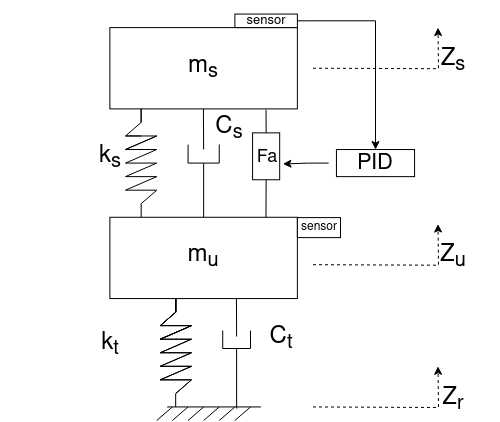
\includegraphics[width=\columnwidth]{images/qcm.png}
    \caption{Two degree of freedom quarter car model with the tire modeled as a spring and a damper.}
    \label{fig:qcm}
\end{figure}

% Newton
The differential equations for a linear model of a quarter car vehicle can be established using Newtons second law of motion and is illustrated in\:\eqref{eq:newton_sprung} and\:\eqref{eq:newton_unsprung}.
\begin{dmath}
    \label{eq:newton_sprung}
    m_s\ddot{z}_s = -k_s(z_s - z_u) - c_s(\dot{z}_s - \dot{z}_u) + F_a
\end{dmath}

\begin{equation}
    \begin{split}
        \label{eq:newton_unsprung}
        m_u\ddot{z}_u = k_s(z_s - z_u) + c_s(\dot{z}_s - \dot{z}_u) \\
        - k_t(z_u - z_r) - c_t(\dot{z}_u - \dot{z}_r) - F_a \\
        = k_s(z_s - z_u) + c_s(\dot{z}_s - \dot{z}_u) \\
        -k_t z_u - c_t\dot{z}_u + F_r - F_a
    \end{split}
\end{equation}

\begin{dmath}
    \label{eq:f_r}
    F_r = k_t z_r + c_t\dot{z}_r
\end{dmath}

% State, input and output
The state vector was defined as the sprung mass vertical displacement and velocity, as well as the unsprung mass vertical displacement and velocity, see\:\eqref{eq:state_vector}.
\begin{equation}
\label{eq:state_vector}
X = 
\begin{bmatrix}
z_s \\
\dot{z}_s \\
z_u \\
\dot{z}_u
\end{bmatrix}
\end{equation}

The input vector was defined as the force from the road and the active control force, see\:\eqref{eq:input_vector} and\:\eqref{eq:f_r}.
\begin{equation}
\label{eq:input_vector}
U = 
\begin{bmatrix}
F_r \\
F_a
\end{bmatrix}
\end{equation}

The output vector was defined as the sprung mass vertical acceleration and velocity, as well as the vertical velocity of the unsprung mass, see\:\eqref{eq:output_vector}.
\begin{equation}
\label{eq:output_vector}
Y = 
\begin{bmatrix}
\ddot{z}_s \\
\dot{z}_s \\
\dot{z}_u
\end{bmatrix}
\end{equation}

% A B C D matrices
From equations [\eqref{eq:newton_sprung},\:\eqref{eq:newton_unsprung},\:\eqref{eq:f_r},\:\eqref{eq:state_vector},\:\eqref{eq:input_vector},\:\eqref{eq:output_vector}],
\begin{comment}
With the states \eqref{eq:state_vector}, inputs \eqref{eq:input_vector}, outputs\:\eqref{eq:output_vector}\:and using\:\eqref{eq:newton_sprung}\:and\:\eqref{eq:newton_unsprung}, and substituting\:\eqref{eq:f_r}\:in\:\eqref{eq:newton_unsprung}, 
\end{comment}
the state space equations can be derived as illustrated in\:\eqref{eq:state_space}.

\begin{dmath}
\label{eq:state_space}
\left\{
\begin{array}{ll}
    \dot{X} = AX + BU \\
    Y = CX + DU
\end{array}
\right.
\end{dmath}

\begin{comment}
\begin{dmath}
    \label{eq:state_space_x}
    \dot{X} = AX + BU
\end{dmath}

\begin{dmath}
    \label{eq:state_space_y}
    Y = CX + DU
\end{dmath}
\end{comment}
The A, B, C and D matrices can then be obtained from the state space equations\:\eqref{eq:state_space} as illustrated in\:\eqref{eq:A_matrix},\:\eqref{eq:B_matrix},\:\eqref{eq:C_matrix} and\:\eqref{eq:D_matrix}.

\begin{equation}
\label{eq:A_matrix}
A = 
\begin{bmatrix}
0 & 1 & 0 & 0 \\
-\frac{k_s}{m_s} & -\frac{c_s}{m_s} & \frac{k_s}{m_s} & \frac{c_s}{m_s} \\
0 & 0 & 0 & 1 \\
\frac{k_s}{m_u} & \frac{c_s}{m_u} & \frac{-k_s-k_t}{m_u} & \frac{c_s-c_t}{m_u}
\end{bmatrix}
\end{equation}

\begin{equation}
\label{eq:B_matrix}
B = 
\begin{bmatrix}
0 & 0 \\
0 & \frac{1}{m_s} \\
0 & 0 \\
\frac{1}{m_u} & -\frac{1}{m_u}
\end{bmatrix}
\end{equation}

\begin{equation}
\label{eq:C_matrix}
C = 
\begin{bmatrix}
-\frac{k_s}{m_s} & -\frac{c_s}{m_s} & \frac{k_s}{m_s} & \frac{c_s}{m_s} \\
0 & 1 & 0 & 0 \\
0 & 0 & 0 & 1
\end{bmatrix}
\end{equation}

\begin{equation}
\label{eq:D_matrix}
D = 
\begin{bmatrix}
0 & \frac{1}{m_s} \\
0 & 0 \\
0 & 0 \\
\end{bmatrix}
\end{equation}
%-------------------------------------------------------------------------------------------------------------
\subsection{Simulation}
% Definiera olika tester för den mekatroniska simuleringen och ange tydligt syftet med varje test och varför det genomförs. Ni ska genom testerna kunna visa att systemet uppfyller de krav och mål ni ställt.

% Parameters
The parameters used for simulation of the quarter car model can be seen in Table.\:\ref{tab:parameters}. The total simulation time used was $200$ seconds. The desired vertical acceleration of the sprung mass was set to zero, $\ddot{z}_{s\_desired} = 0 \frac{\text{m}}{\text{s}^2}$.
\begin{table}[ht]
	\centering
	\begin{tabular}{|l|l|l|l|l|l|}
			\hline
			Symbol       & Value     & Unit                                         \\
			\hline
			$m_s$        & $86.5$    & $\text{kg}$                                  \\
			$m_u$        & $9.2$     & $\text{kg}$                                  \\
            $k_s$        & $4550$    & $\frac{\text{N}}{\text{m}}$                  \\
            $k_t$        & $150000$  & $\frac{\text{N}}{\text{m}}$                  \\
            $c_s$        & $300$     & $\text{N}\cdot\frac{\text{s}}{\text{m}}$     \\
            $c_t$        & $45$      & $\text{N}\cdot\frac{\text{s}}{\text{m}}$     \\
            $n$          & $0.94$    & Ratio                                        \\
			\hline
		\end{tabular}
	\caption{Parameter values used for simulation. Estimated based on\:\cite{mdhsolarteamBillMaterials}\cite{cfw16inchTypeC}.}
	\label{tab:parameters}
\end{table}

% Energy, actuator/generator control
The control between generator and actuator modes were implemented using Stateflow, see Fig.\:\ref{fig:stateflow_chart} (note that integration was done outside the Stateflow chart). The system enters actuator mode when $ (\dot{z}_s - \dot{z}_u) > 0$ which means that the sprung mass is moving faster than the unsprung mass and requires damping. The system enters generator mode when $ (\dot{z}_s - \dot{z}_u) \le 0$, and thus harvests the energy provided by the relative motion when the unsprung mass is moving faster than the sprung mass. The formula for energy consumed can be seen in\:\eqref{eq:consumed} and the energy regenerated can be seen in\:\eqref{eq:regenerated}, similar to\:\cite{yinPerformanceEvaluationActive2015}. The fraction $\frac{1}{n}$ in\:\eqref{eq:consumed} was the result of the motor efficiency in actuator mode acting on the energy consumed $n \cdot W_c$, and thus transferring it over to the right hand side results in division. In generator mode\:\eqref{eq:regenerated} it is the opposite, the motor efficiency acts on the work which drives the generator.
\begin{center}
    \begin{equation}
        \begin{split}
            \label{eq:consumed}
            W_c = \int_{0}^{t} \frac{F_a}{n} \cdot (\dot{z}_s - \dot{z}_u), \: F_a \cdot (\dot{z}_s - \dot{z}_u) \le 0
        \end{split}
    \end{equation}
\end{center}
\begin{center}
    \begin{equation}
        \begin{split}
            \label{eq:regenerated}
            W_r = \int_{0}^{t} n \cdot F_a \cdot (\dot{z}_s - \dot{z}_u), \: F_a \cdot (\dot{z}_s - \dot{z}_u) \ge 0
        \end{split}
    \end{equation}
\end{center}
The total energy gained or consumed by the actuator was then calculated by\:\eqref{eq:actuator_energy}.
\begin{equation}
    \label{eq:actuator_energy}
    W_{total} = W_c + W_r
\end{equation}
\begin{figure}
    \centering
    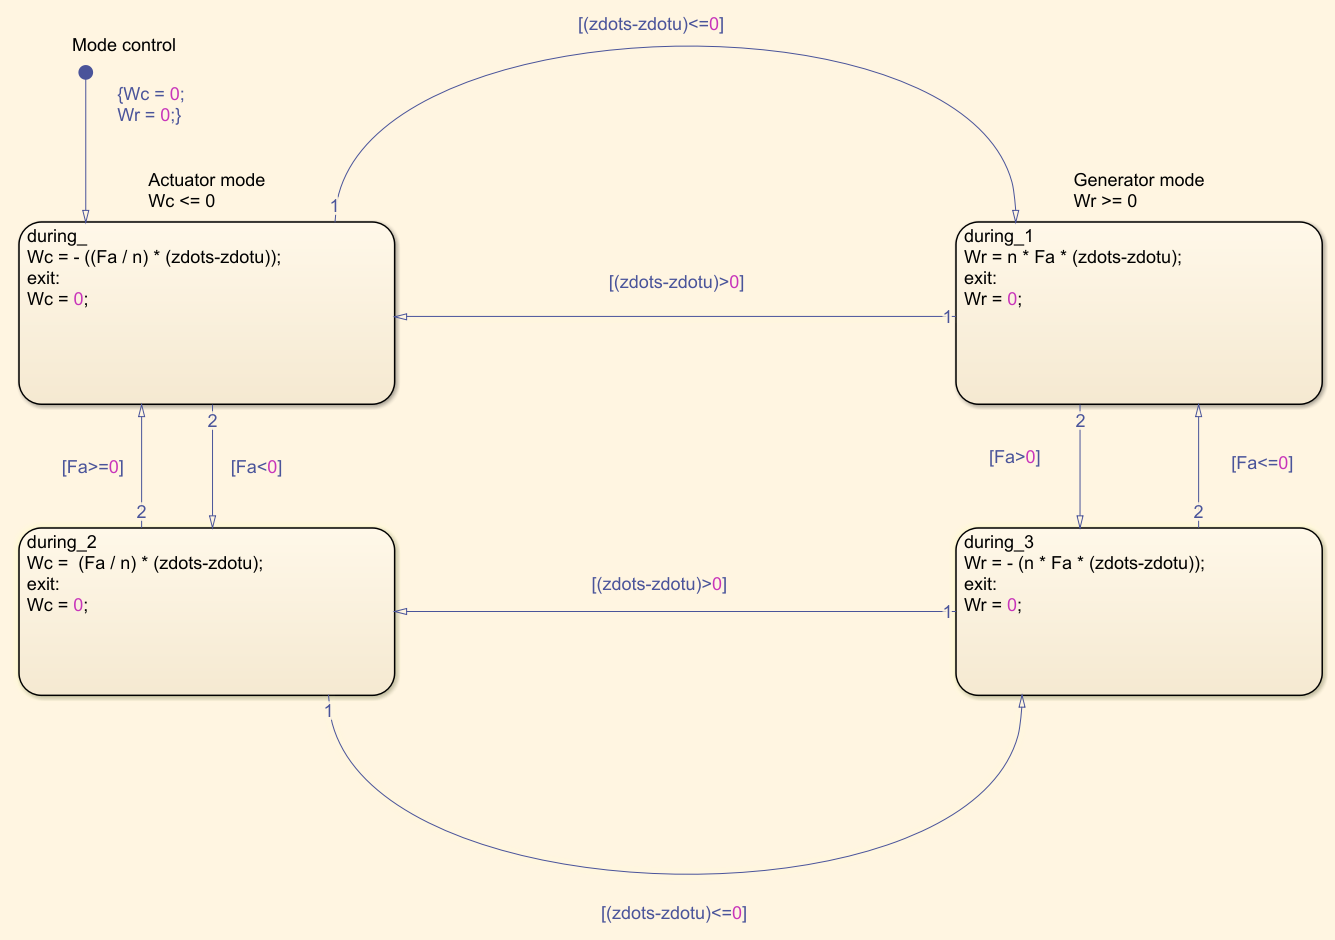
\includegraphics[width = \columnwidth]{images/stateflow_chart.png}
    \caption{The Stateflow chart which controls the switching between generator and actuator modes. Note that the integration part of the equation for energy consumed and regenerated was done outside the Stateflow chart.}
    \label{fig:stateflow_chart}
\end{figure}
The self supplying efficiency, $n_{ss}$, was defined as the fraction of energy regenerated to energy consumed, see\:\eqref{eq:self_supplying_efficiency}.
\begin{dmath}
    \label{eq:self_supplying_efficiency}
    n_{ss} = \frac{|W_r|}{|W_c|}
\end{dmath}

% PID
A PID controller was used to minimize the error which was the deviation of actual value from the setpoint. The setpoint was the desired vertical acceleration of the sprung mass $\ddot{z}_{s\_desired} = 0\frac{\text{m}}{\text{s}^2}$. The actual value was the first component of the output vector, $\ddot{z}_s$, this was provided by the negative feedback. See Fig.\:\ref{fig:simulink_diagram} for the complete simulation block diagram in Simulink (note that the time dependency of variables has been excluded to help minimize cluttering). The final PID controller values were: $P = 500$, $I = 5$, $D = 1$, taken from\:\cite{liuModelingSimulationEnergyRegenerative2019}.
\begin{figure}
    \centering
    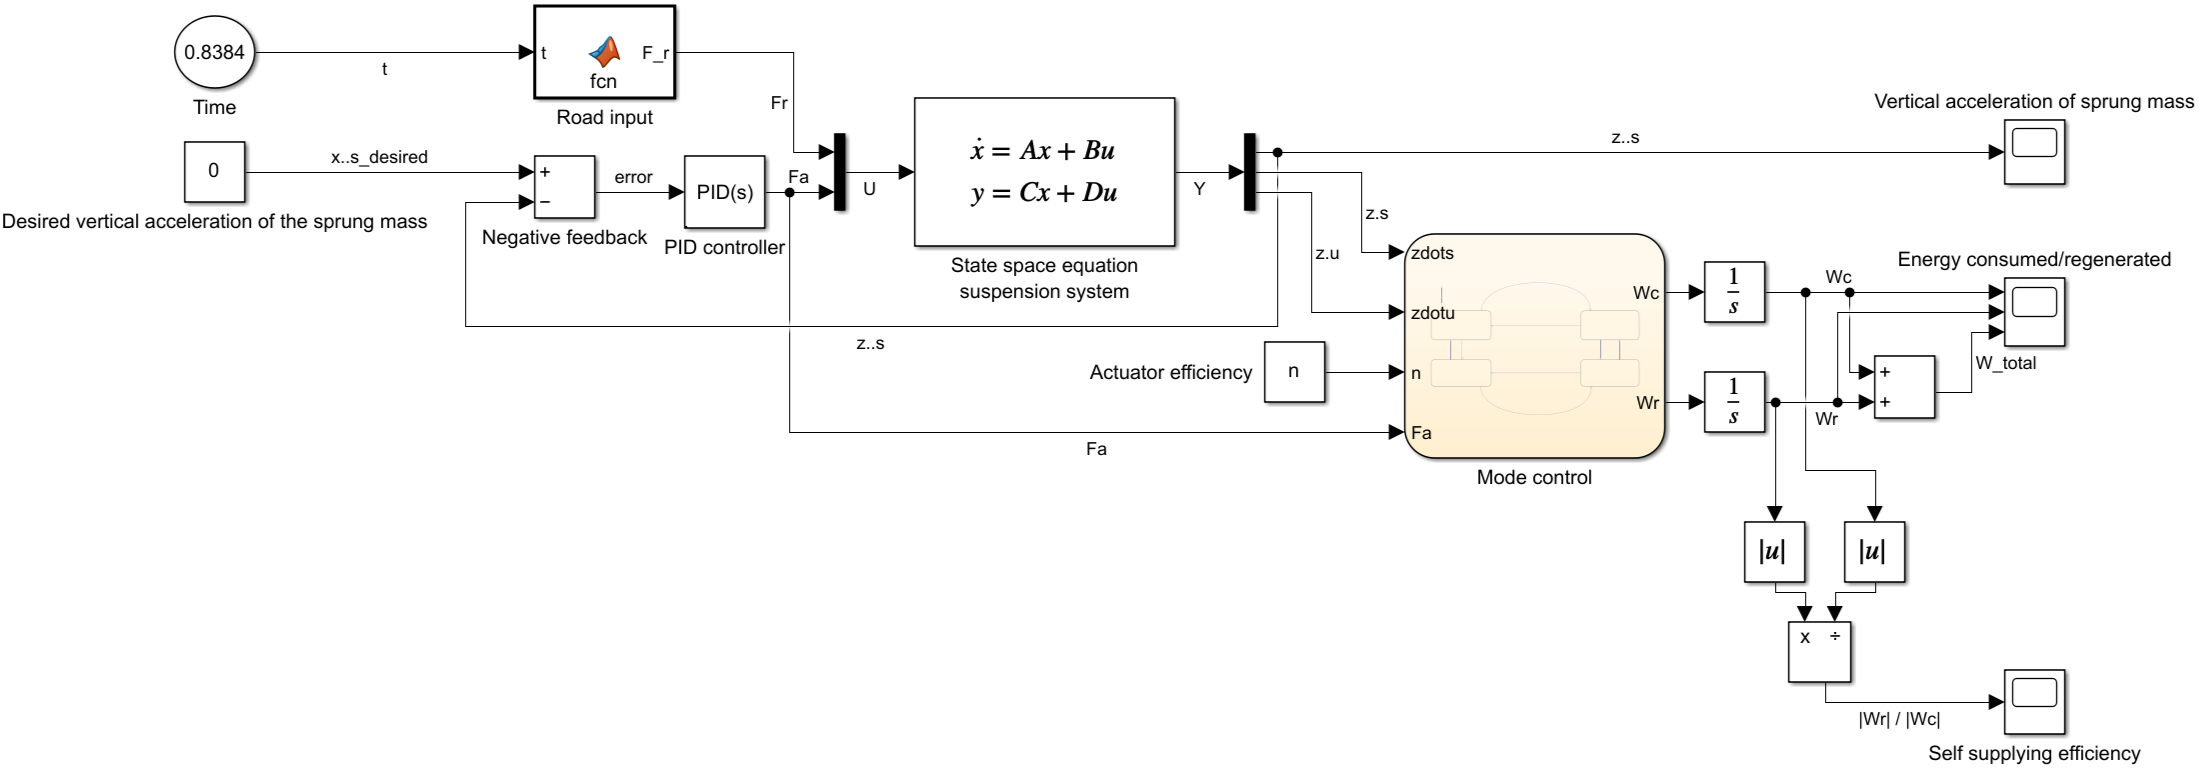
\includegraphics[width=\columnwidth]{images/simulink_diagram.png}
    \caption{The complete block diagram in Simulink. Note that the time dependency of variables has been excluded to help minimize cluttering.}
    \label{fig:simulink_diagram}
\end{figure}

% Tests
For the tests, a random road model was created, which consisted of applying different types of noise (random road input) to the road input to simulate different types of road conditions and speeds. The random road model can be seen in\:\eqref{eq:noise}.
\begin{dmath}
    \label{eq:noise}
    F_r = | a_1 \cdot sin(f_1 \cdot t + p_1) + a_2 \cdot cos(f_2 \cdot t + p_2) |
\end{dmath}
The tests were performed with the purpose of verifying the system and ensuring road comfort was maintained and evaluating the system based on the performance metrics. The different tests can be seen in Table.\:\ref{tab:tests}. It should be noted that the test names are not absolute, a test which was named as a certain speed can also be considered as a lower speed but worse road condition.
\begin{table}[ht]
	\centering
	\resizebox{\columnwidth}{!}{\noindent\begin{tabular}{|l|l|l|l|l|l|l|l|}
			\hline
			Test                                     & $t$ (s)           & $a_1$ (N)     & $f_1$ (Hz)    & $p_1$ (rad)    & $a_2$ (N)        & $f_2$ (Hz)     & $p_2$ (Rad)      \\
			\hline
			Speed bump                               & 10, 40, 80, 90    & 0             & 0             & 0              & [200000 400000]  & 0              & 0                \\
			$0-10\frac{\text{km}}{\text{h}}$         & [0 10)            & [0 1000]      & [0 2]         & [0 1]          & [0 1000]         & [0 2]          & [0 1]            \\
            $10-20\frac{\text{km}}{\text{h}}$        & (10 20)           & [0 4000]      & [1 3]         & [0 1]          & [0 4000]         & [1 3]          & [0 1]            \\
            $20-30\frac{\text{km}}{\text{h}}$        & (20 30)           & [0 6000]      & [3 5]         & [0 1]          & [0 6000]         & [3 5]          & [0 1]            \\
            $30-40\frac{\text{km}}{\text{h}}$        & (30 40)           & [0 9000]      & [4 6]         & [0 1]          & [0 9000]         & [4 6]          & [0 1]            \\
            $40-50\frac{\text{km}}{\text{h}}$        & (40 50)           & [0 11000]     & [6 8]         & [0 1]          & [0 11000]        & [6 8]          & [0 1]            \\
            $50-60\frac{\text{km}}{\text{h}}$        & (50 60)           & [0 13000]     & [7 9]         & [0 1]          & [0 13000]        & [7 9]          & [0 1]            \\
            $60-70\frac{\text{km}}{\text{h}}$        & (60 70)           & [0 16000]     & [9 11]        & [0 1]          & [0 16000]        & [9 11]         & [0 1]            \\
            $70-80\frac{\text{km}}{\text{h}}$        & (70 80)           & [0 18000]     & [10 12]       & [0 1]          & [0 18000]        & [10 12]        & [0 1]            \\
            $80-90\frac{\text{km}}{\text{h}}$        & (80 90)           & [0 21000]     & [12 14]       & [0 1]          & [0 21000]        & [12 14]        & [0 1]            \\
            $90-100\frac{\text{km}}{\text{h}}$       & (90 100)          & [0 23000]     & [14 16]       & [0 1]          & [0 23000]        & [14 16]        & [0 1]            \\
            $100-110\frac{\text{km}}{\text{h}}$      & (100 150)         & [0 26000]     & [15 17]       & [0 1]          & [0 26000]        & [15 17]        & [0 1]            \\
            Rest                                     & (150 $\infty$)      & 0             & 0             & 0              & 0                & 0              & 0                \\
			\hline
		\end{tabular}}
	\caption{Description of all the tests for the system. Test names can also be considered as a lower speed but worse road condition.}
	\label{tab:tests}
\end{table}

%-------------------------------------------------------------------------------------------------------------
\subsection{Design}
% Konstruera en teoretisk systemdesign och motivera den med hänsyn till resultaten från modellen och simuleringen.
A theoretical system design for the proposed RASS model was created. Important considerations for its viability and integration with the MDH solar car were also covered. Unfortunately, because of the insufficient documentation of the MDH solar car, an actual theoretical system design was not relevant since it would require to many assumptions. Therefor this section describes considerations for a theoretical system design if proper information was available.
\subsubsection{Sensors}
The proposed system requires two types of sensors: accelerometers and velocity sensors.
An accelerometer is necessary for monitoring the vertical acceleration of the sprung mass, which is used by the active suspension control. Dual accelerometers (redundancy) would be placed in each wheelhouse as close to the wheel as possible.

The use of a pair of velocity sensors, dual sensors in the wheel and dual sensors in the wheelhouse (redundancy), for each wheel of the car is necessary for mode control and calculating the energy regenerated and consumed by the RASS, see\:\eqref{eq:consumed} and\:\eqref{eq:regenerated}.
Both the accelerometers and velocity sensors must be resistant to vibration, liquid and smaller impacts from objects like gravel. Possible accelerometer options include MEMS or piezoelectric sensors. Some velocity sensors which might work well include hall effect sensors or piezoelectric velocity sensors.
However the final choice of sensors must be done after substantial testing, once proper functioning with the rest of the system and electrical network has been ensured, as well as final cost considerations.

\subsubsection{Actuator and generator}
The use of a DC motor as the actuator for a RASS is common and it can function as both actuator and generator\:\cite{liuTransmissionEnergyharvestingStudy2021}\cite{liuModelingSimulationEnergyRegenerative2019}\cite{zhengNovelEnergyregenerativeActive2008}. The choice of a DC motor thus serves as a good outset option for the initial theoretical system design. 
Brushless DC motors are common options\:\cite{zhengNovelEnergyregenerativeActive2008}, especially permanent magnet brushless DC motors\:\cite{liuTransmissionEnergyharvestingStudy2021}\cite{liuModelingSimulationEnergyRegenerative2019}\cite{yongchaozhangExperimentalVerificationEnergyregenerative2007}, a permanent magnet brushless DC motor was therefor chosen. 
One actuator/generator is required for each wheel, and thus one motor for each wheel. This will result in significant cost and power requirements. Thus the final choice of motor must consider even more so the energy consumption characteristics of the motor as well as the cost, along with other important considerations like torque and its ability to be integrated with the control electronics and the feedback system.
The final choice of permanent magnet brushless DC motor is thus very complex since it must integrate well with the existing electronics and systems of the MDU solar car.

\subsubsection{Control systems}
A number of control systems are necessary for the RASS to function, including: mode control, active suspension control and energy control. All control units would be implemented as dual units because of redundancy. 
The mode control uses the velocity sensor values and is necessary to switch between the actuator mode and generator mode since both can not be used at the same time. One mode control unit is required for each actuator, the mode control was implemented as a Stateflow chart in the simulations. The mode control unit would most likely be an embedded system with a real-time operating system (RTOS).
The active suspension control uses the accelerometer values to regulate the active control force to minimize sprung mass vertical acceleration. The active suspension control was implemented as a PID controller in the Simulink simulations. One active suspension control unit is required per wheelhouse. The active suspension control unit would much like the mode control unit most likely be implemented as an embedded system using a RTOS.
The power management and battery management systems and controllers need to be expanded to allow for the regenerative part of the RASS system to function and be integrated. Proper management of the energy harvested and how it should be stored, optimization of energy regeneration and power delivery to the actuator are some of the important aspects related to the different management systems.

\subsubsection{Energy storage}
The use of capacitors or ultra capacitors could improve energy regeneration and provide more optimal utilization of the energy harvested from the RASS, much like it does for regenerative braking (see Introduction\:\ref{section:intro}), but would increase the initial cost of the system. However for this initial theoretical system design, this was skipped for simplicity, and all energy storage needs would be handled by the batteries.

%batteries?

\subsubsection{Power electronics}
The RASS requires converters for converting the electricity from storage to actuator and from generator to storage.
For storage to actuator this would roughly be a DC-DC converter from $126\:\text{V}$\:\cite{mdhsolarteamBillMaterials} to $12-48\:\text{V}$ (depending on motor and the required output torque).
Also, the generated energy needs to be stepped up by a DC-DC converter to be able to be stored in the $126\:\text{V}$ battery\:\cite{mdhsolarteamBillMaterials}.

\subsubsection{Integration}
Integrating the RASS with the MDH solar car requires several considerations. One such consideration is the mass distribution, this is especially important since the MDH solar car uses in-wheel drive and thus a lot of the mass is unsprung mass. A low unsprung mass would mean less force is transmitted to the sprung mass increasing ride comfort. As mentioned previously, the model assumes all wheels have equal mass and are identical, this is however not the case in reality, the rear wheels have significantly more mass because of in-wheel configuration in only the rear wheels. Therefor, a proper model should be implemented covering all four wheels of the car taking the differences in mass into account. The majority of the mass of the RASS should also be attempted to be anchored in the sprung mass, for example the heavier side of the damper, to prevent increasing unsprung mass.
Integrating the RASS into the current electrical network and the current suspension system of the car is also tricky.
Considerations such as whether sufficient power can be provided to the RASS given the current electrical network, additional load and possible impact on the performance given increased power demands and possible electromagnetic compatibility (EMC) issues.
Considerations regarding integrating the RASS with the current suspension system was not possible because of the insufficient documentation of the current suspension system. However, possible considerations include space and changes of the passive springs and dampers.

\subsubsection{Safety}
Redundancy would be used to ensure the system does not stop functioning or become unsafe if a part of the RASS stops being operational. This includes: dual sensors, dual communications channels, dual control units, redundant feedback systems, springs and actuators with redundancy if one fails, additional or emergency power supply if main power supply fails, multiple algorithms and using voting between them.
The proposed theoretical system requires significant testing to ensure it meets its functional requirements and is safe.

\subsubsection{User interface}
A user interface to allow proper view of the system status and user control of the system. A user interface would in turn require a controller and would probably be implemented using a design pattern like model view presenter (MVP) and running a RTOS.

\subsubsection{Performance tuning}
The control algorithms would require performance tuning to function optimally. This would include global optimization and real time optimization\:\cite{carlenerikssonEVHEVFramdrivning2023}. Updates to the control algorithms is also necessary to consider in case of faults and improvements.

\subsubsection{Regulatory compliance}
Regulations and standards for suspension systems were unavailable because of the cost of access to such documents. However it is paramount that such standards are followed and the regulations obeyed.

\subsubsection{Mass}
As previously noted, the system design must not cause mass distribution problems nor increase the vehicles mass above a certain limit. This could not be assessed since information regarding mass was not available.
%This is not expected to be a problem for the proposed RASS. 

\subsubsection{Dimension}
The system must also have viable dimensions to fit the MDH solar car. This could not be established properly since proper information was not available.

\subsubsection{Cost}
The cost of the system is one of the most important aspects, however, since no budget was available, this could not be evaluated.



%-------------------------------------------------------------------------------------------------------------
% Översätt den valda designen till eventuella arbetsritningar, kretsscheman, etc.
% Ritningar och en materialförteckning (BoM) för systemet med en tydlig motivering
% CAD?

A flowchart describing the theoretical system design and the workings of the model can be seen in Fig.\:\ref{fig:RASS_flowchart}. The user interface and some other interactions were excluded from the flowchart shown in Fig.\:\ref{fig:RASS_flowchart}, because the focus was on the suspension part of the system.

\begin{figure}
    \centering
    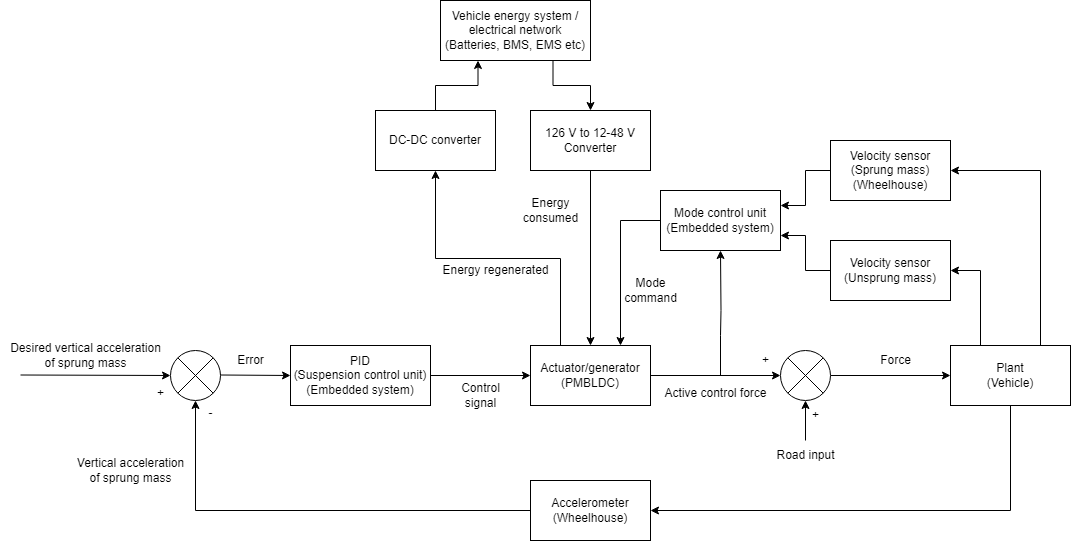
\includegraphics[width=\columnwidth]{images/RASS_flowchart.png}
    \caption{RASS flowchart describing the theoretical system design and its functionality. Note that some interactions and the user interface has been excluded since the focus was on the suspension part of the system.}
    \label{fig:RASS_flowchart}
\end{figure}

%-------------------------------------------------------------------------------------------------------------
\section{Results}
%-------------------------------------------------------------------------------------------------------------
% Acceleration
The vertical acceleration of the sprung mass $\Ddot{z}_s$ remained below $1.5\frac{\text{m}}{\text{s}^2}$ during the entire simulation except for two spikes at the very roughest parts (see Table.\:\ref{tab:tests}), see Fig.\:\ref{fig:vertical_acceleration}.
\begin{figure}
    \centering
    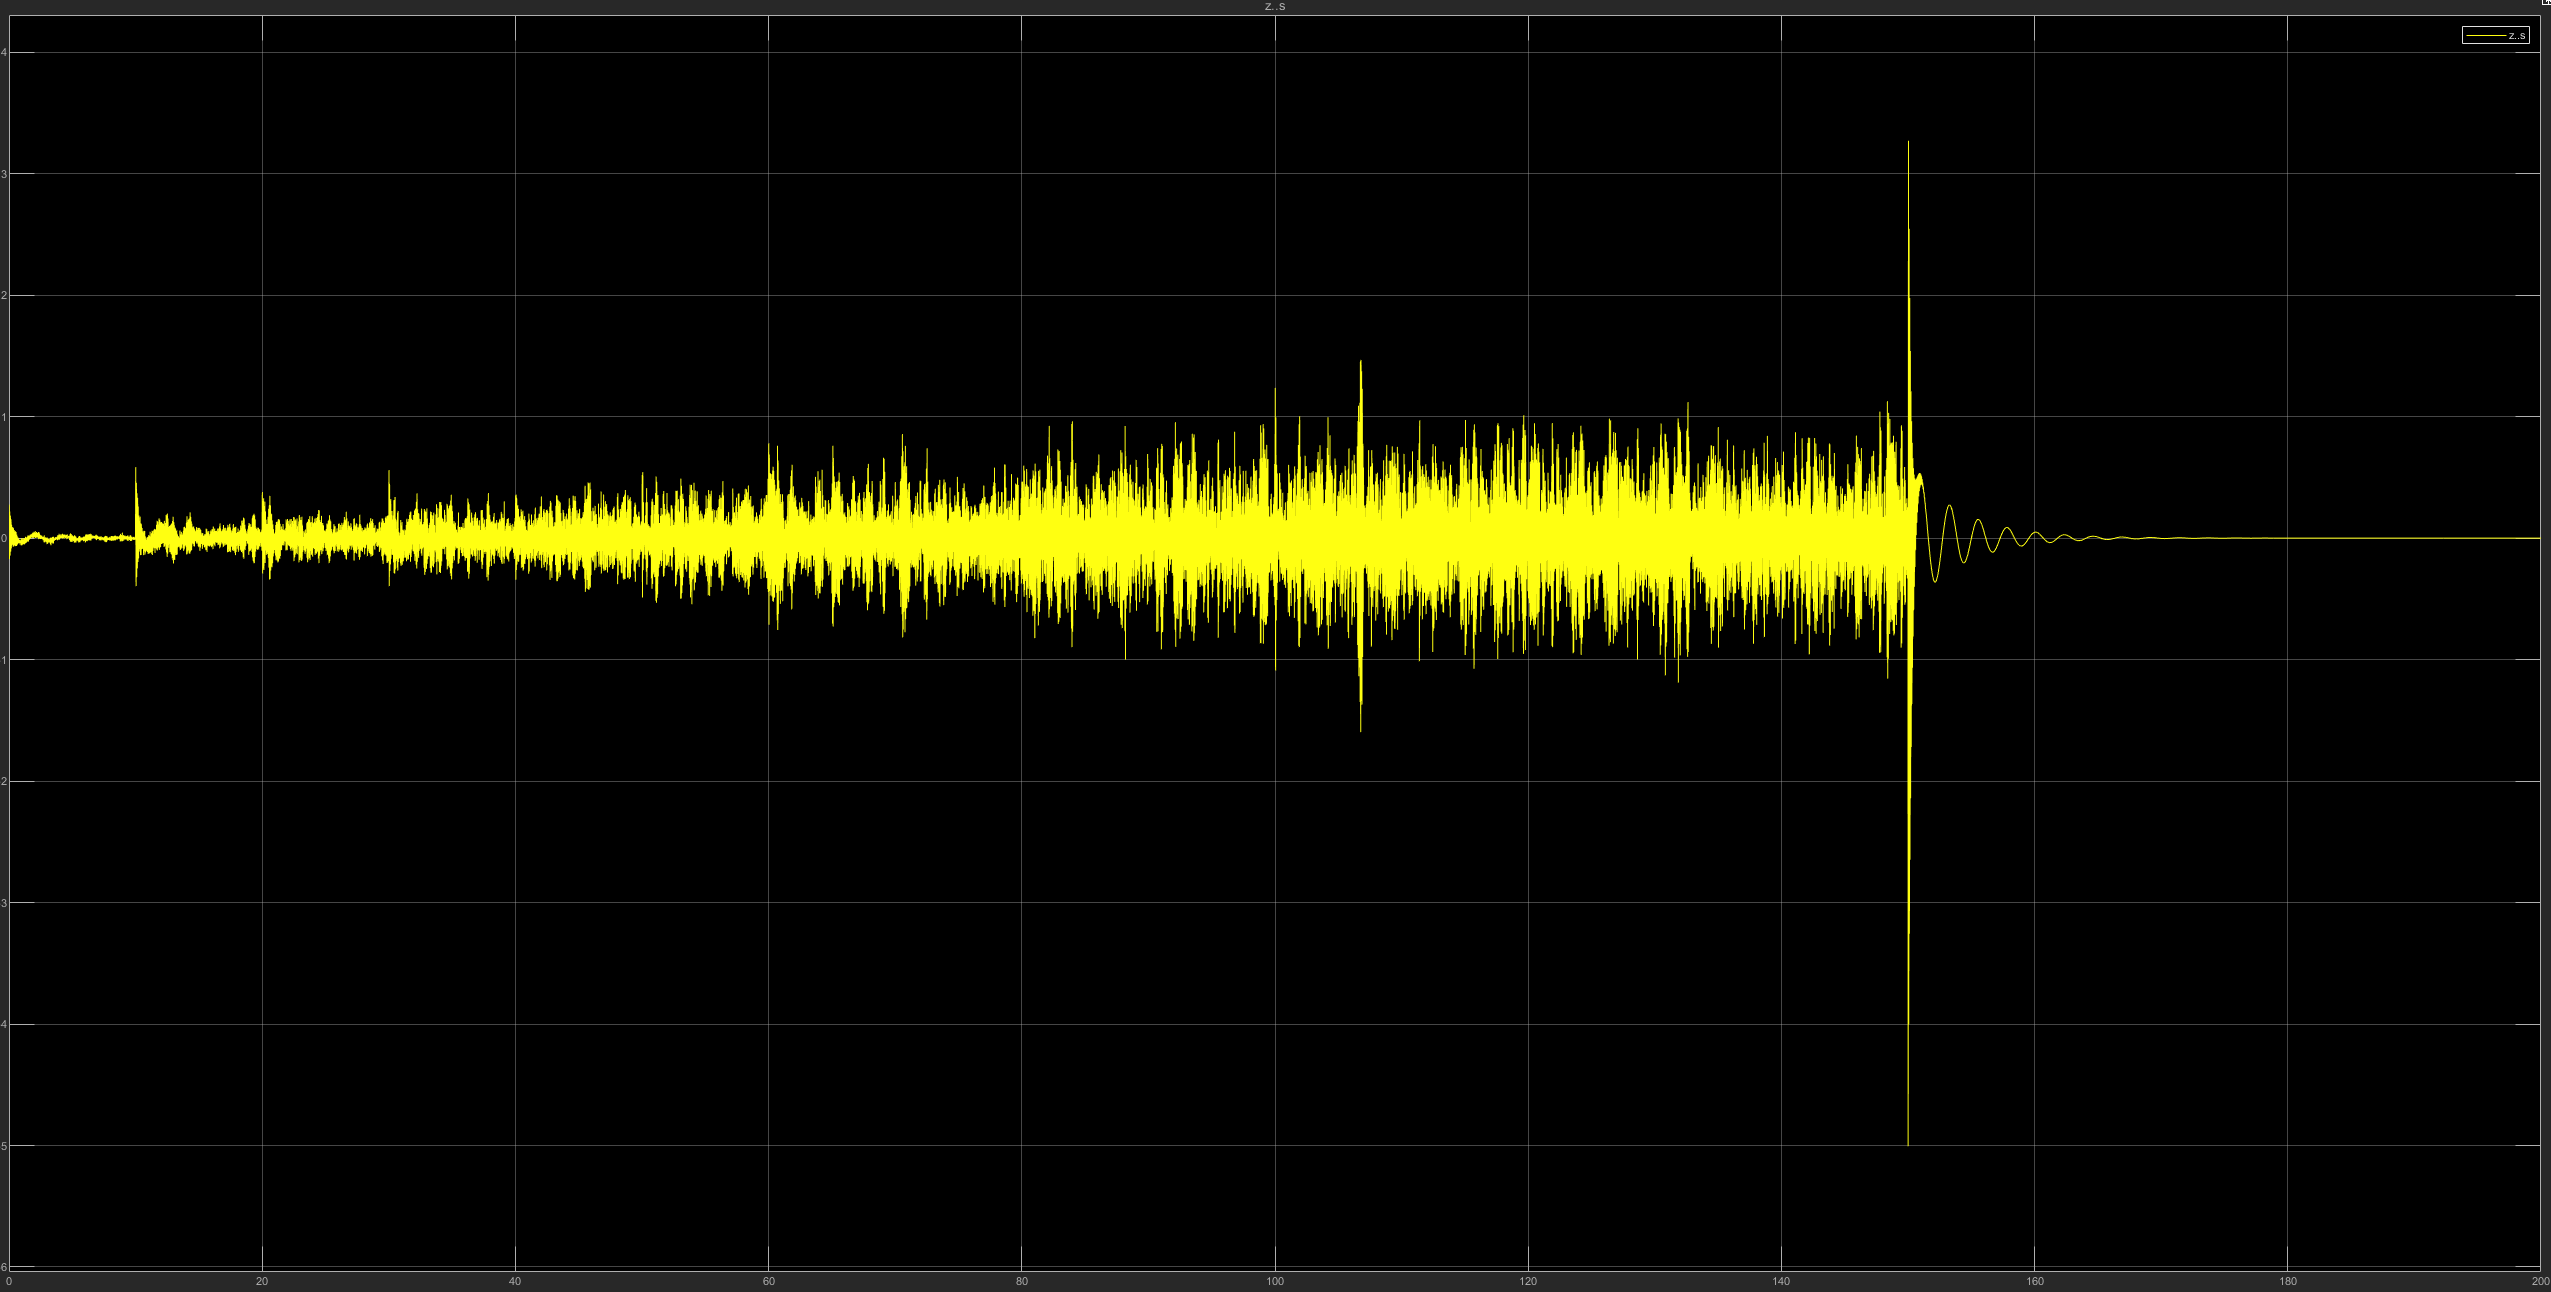
\includegraphics[width=\columnwidth]{images/vertical_acceleration.png}
    \caption{Simulation results of the vertical acceleration of the sprung mass.}
    \label{fig:vertical_acceleration}
\end{figure}

% Energy
The energy results obtained, when the simulated model was subjected to the noise input described in \eqref{eq:noise} and Table.\:\ref{tab:tests}, can be seen in Table.\:\ref{tab:results_energy}, Fig.\:\ref{fig:energy_results_graph} and Fig.\:\ref{fig:self_supplying}.
\begin{table}[ht]
	\centering
	\begin{tabular}{|l|l|l|l|l|l|}
			\hline
			Metric                                            & Proposed RASS        \\
			\hline
			Energy consumed (J)                               & $-6760$               \\
			Energy regenerated (J)                            & $5650$               \\
			Total energy consumed/regenerated (J)             & $-1110$               \\
            Self supplying efficiency (\%)                    & $88$             \\
			\hline
		\end{tabular}
	\caption{All energy values obtained from the simulation.}
	\label{tab:results_energy}
\end{table}

\begin{figure}
    \centering
    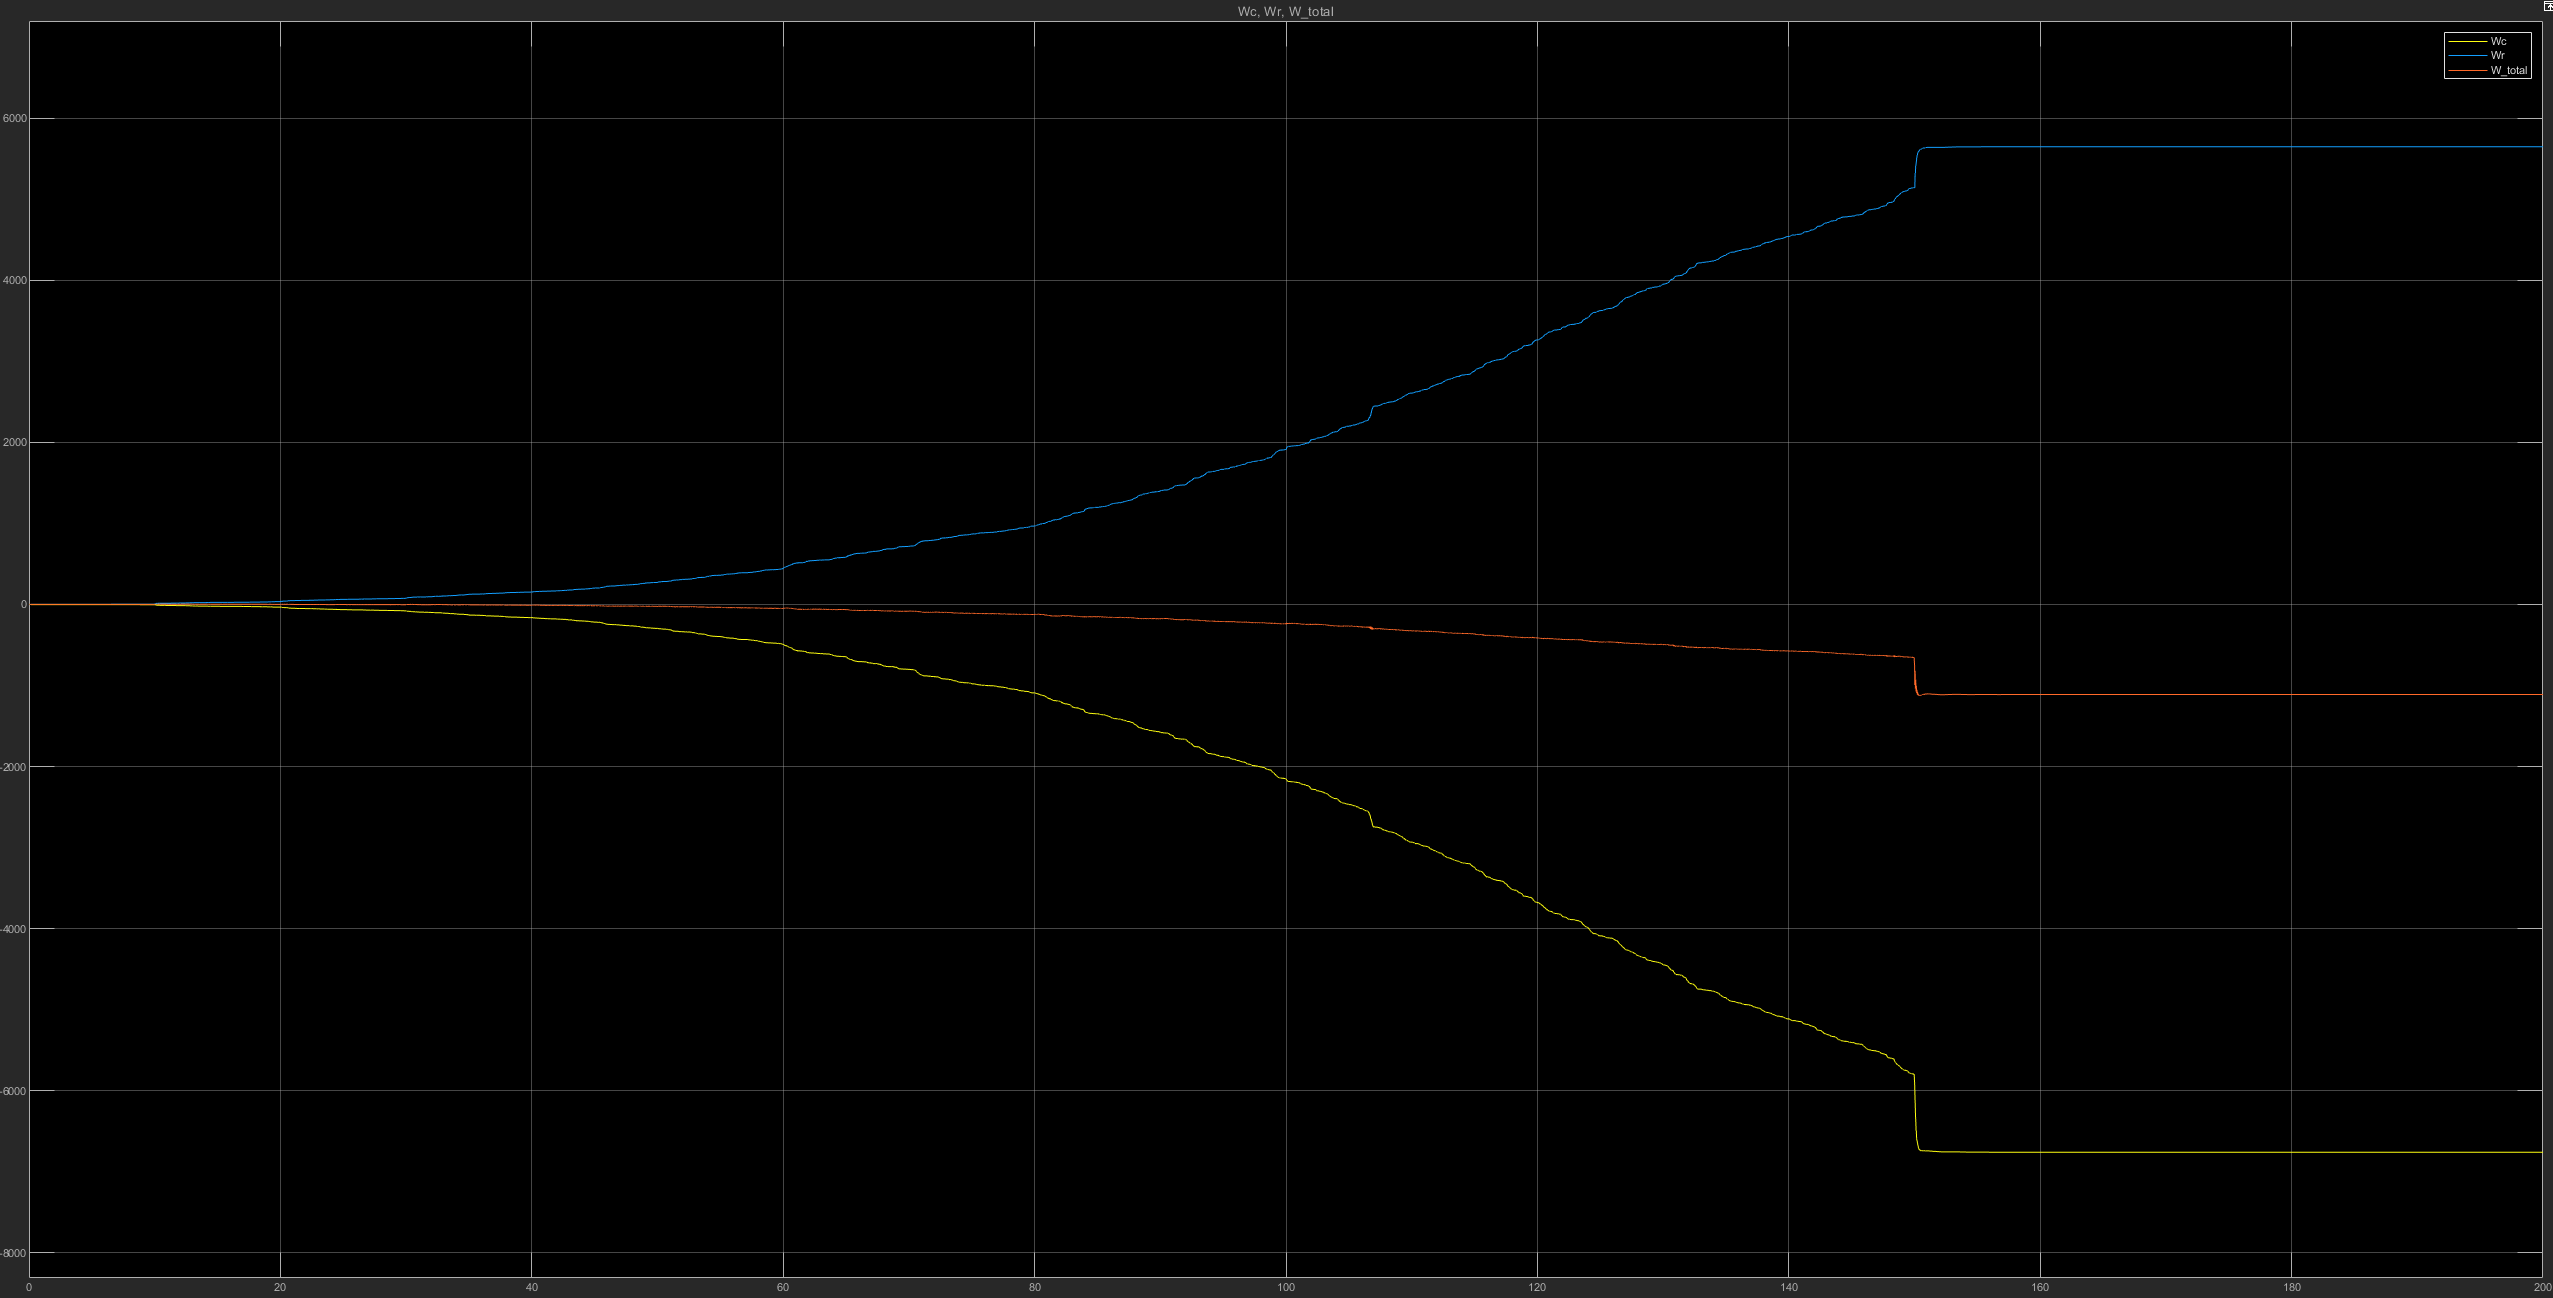
\includegraphics[width=\columnwidth]{images/energy_results.png}
    \caption{Simulation results of the energy consumed, regenerated and total energy. Yellow line is energy consumed, blue line is energy regenerated and red line is total energy.}
    \label{fig:energy_results_graph}
\end{figure}

\begin{figure}
    \centering
    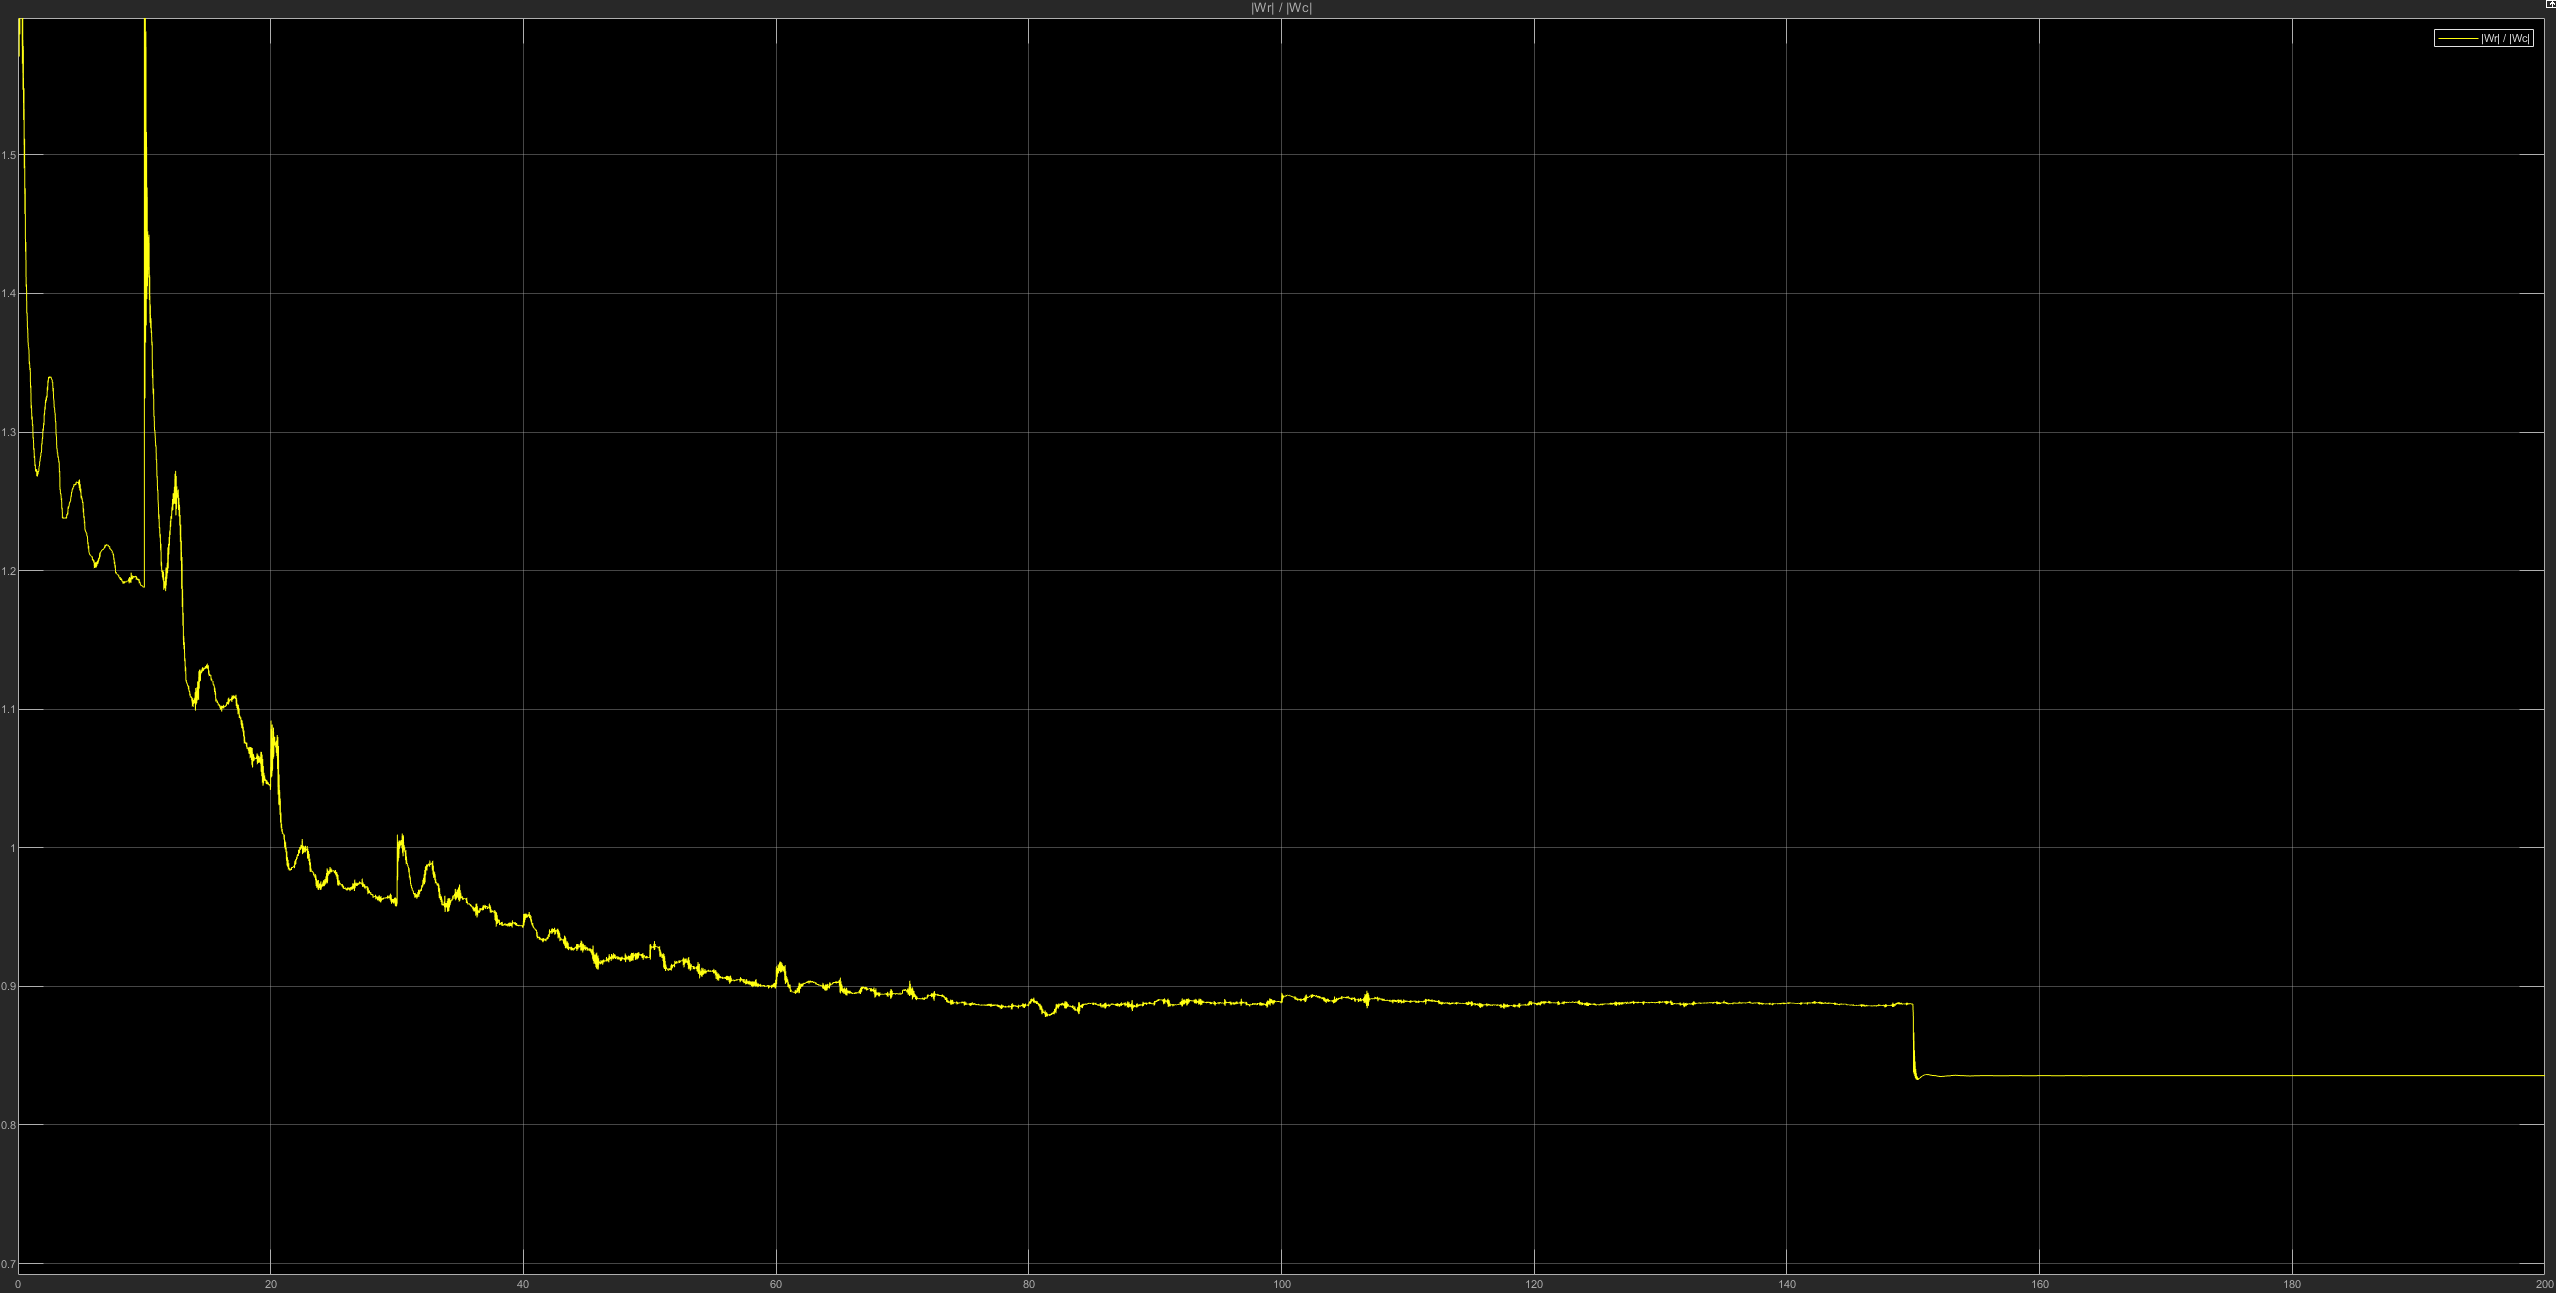
\includegraphics[width=\columnwidth]{images/self_supplying.png}
    \caption{Simulation results of the self supplying efficiency.}
    \label{fig:self_supplying}
\end{figure}

A number of requirements could not be evaluated, including energy efficiency.
%-------------------------------------------------------------------------------------------------------------
\section{Discussion}
\label{section:discussion}
%-------------------------------------------------------------------------------------------------------------

% Results 
The modeled mechanical behavior of the system was satisfactory and match other studies, mainly based on sprung mass acceleration\:\cite{liuTransmissionEnergyharvestingStudy2021}, see Fig.\:\ref{fig:vertical_acceleration}. It is seen as satisfactory since the two peaks exceeding $1.5\frac{\text{m}}{\text{s}^2}$ are during harsher conditions than described in other studies\:\cite{liuTransmissionEnergyharvestingStudy2021}.
However, the energy results obtained were clearly unrealistic when compared to other studies, mainly self supplying efficiency\:\cite{azmiNovelOptimalControl2023}\cite{liuTransmissionEnergyharvestingStudy2021}\cite{liuModelingSimulationEnergyRegenerative2019}, see Fig.\:\ref{fig:self_supplying} and Table.\:\ref{tab:results_energy}.
One reason for this was the inadequate incorporation of losses and efficiency, only motor efficiency was part of the simulation model.
Another contributing factor was that the parameters were only poor estimations, a consequence of poor documentation of the MDH solar car, and the results were thus affected by this fault in the model.
System constrains were also not considered, such as maximum actuator force and maximum displacements.
The logic used for mode control was very rudimentary as well, substantial optimization could be done, see\:\cite{azmiNovelOptimalControl2023}.

%-------------------------------------------------------------------------------------------------------------

% Limitations
An additional limitation of this study was that the system did not account for non linear motion and it only made use of linear motion for harvesting energy, as noted in\:\cite{azmiNovelOptimalControl2023}, this significantly reduces the amount of energy which can be harvested.
The model created assumes linear characteristics, however in reality, the characteristic are non linear, this assumption results in worse performance of the controllers and system response\:\cite{azmiNovelOptimalControl2023}. 
The model also assumed all wheels had equal mass and were identical, this is not true for the MDH solar car, something which has already been stated.

%-------------------------------------------------------------------------------------------------------------

% Requirements
Because of the time and resource limitation of this study, most system requirements were unable to be tested, these were marked with "UNKNOWN". However it is imperative that these requirements are tested, all of the requirements established can be tested with proper resources. Hence the reason they were established despite not being able to be tested in this study.
It should also be noted that most of the system requirements were also unable to be properly established because of the limited resources, like lack of proper documentation, these were also marked with "UNKNOWN".
The two requirements which could be tested, ride comfort technically failed, and self supplying efficiency passed, however both of these are misleading given the limitations of the study and the faults presented above.

%-------------------------------------------------------------------------------------------------------------

% Advantage of the results related to MDH solar car
The results obtained, ignoring the unrealistic energy values, indicates a possibly very beneficial system for the MDH solar car. Providing improved suspension characteristics while also reducing the major drawback of active suspension systems. This is especially important given the substantial unsprung mass, because of the in-wheel configuration, and thus the negative effects this has on the suspension system\:\cite{yinPerformanceEvaluationActive2015}, as previously noted in the Introduction\:\ref{section:intro}.

%-------------------------------------------------------------------------------------------------------------


%-------------------------------------------------------------------------------------------------------------
\begin{comment}
% Hur fördelaktigt kan det resulterande systemet vara för MDH solar car?
\end{comment}
%-------------------------------------------------------------------------------------------------------------
\section{Conclusion}
%-------------------------------------------------------------------------------------------------------------

The RASS system developed in this study provides a foundational proof of concept, presenting an initial demonstration of the viability and potential benefits of implementing a RASS for the MDH solar car, and other EVs. Although the study was constrained by the limitations of the study and the information available, it does show sufficient promise for further exploration and research efforts.

%-------------------------------------------------------------------------------------------------------------
\section*{Acknowledgment}
%-------------------------------------------------------------------------------------------------------------

The authors would like to thank Daniel Morberg and Gabriele Gualandi for their support and input on the model developed in this paper.

%The authors would like to thank ... for his/her/their help and support during the process of writing this paper. 
%-------------------------------------------------------------------------------------------------------------
% Select the IEEEtran style
\bibliographystyle{IEEEtran}
% Include bibliography file
\bibliography{ELA306}
\end{document}